\documentclass{standalone}
\usepackage{tikz}
\begin{document}
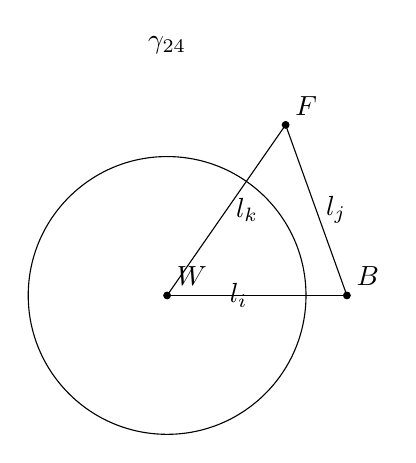
\begin{tikzpicture}[scale=0.6]
  \filldraw (0.0, 0.0) circle (2pt) node[above right] {$W$};
  \filldraw (2.5083, 3.6102) circle (2pt) node[above right] {$F$};
  \filldraw (3.8057, 0.0) circle (2pt) node[above right] {$B$};
  \draw (0.0, 0.0) -- (2.5083, 3.6102) node[midway, right] {$l_k$};
  \draw (3.8057, 0.0) -- (2.5083, 3.6102) node[midway, right] {$l_j$};
  \draw (3.8057, 0.0) -- (0.0, 0.0) node[midway, left] {$l_i$};
  \draw (0.0, 0.0) circle (2.9397) node[above=2.9397cm] {$\gamma_{24}$};
\end{tikzpicture}
\end{document}